\documentclass[12pt,letterpaper,noanswers]{exam}
\usepackage[usenames,dvipsnames,svgnames,table]{xcolor}
\usepackage[margin=0.9in]{geometry}
\renewcommand{\familydefault}{\sfdefault}
\usepackage{multicol}
\usepackage{wrapfig}
\pagestyle{head}
\definecolor{c03}{HTML}{FFDDDD}
\header{AM 22b Class 29}{}{Apr 9: Divergence theorem and curl, p.\thepage}
\runningheadrule
\headrule
\usepackage{graphicx} % more modern
\usepackage{amsmath} 
\usepackage{amssymb} 
\usepackage{hyperref}
\usepackage{tcolorbox}
\usepackage[utf8]{inputenc}
\usepackage{diagbox}
\usepackage{graphicx} 
\usepackage{enumitem}
\usepackage{tikz}
\tikzstyle{startstop} = [rectangle, rounded corners, minimum width=3cm, minimum height=1cm,text centered, draw=black]

\tikzstyle{process} = [rectangle, minimum width=3cm, minimum height=1cm, text centered, draw=black, fill=gray!20]
\tikzstyle{decision} = [ellipse, minimum width=3cm, minimum height=0.5cm, text centered, draw=black, fill=white!30]
\tikzstyle{arrow} = [thick,->,>=stealth]
\usetikzlibrary{shapes.geometric, arrows}
\pagenumbering{arabic}

\usepackage[numbered,autolinebreaks,useliterate]{mcode}

\newcommand{\mb}[1]{\underline{#1}}

\begin{document}
 \pdfpageheight 11in 
  \pdfpagewidth 8.5in




% I need to review the torus trajectories...

\begin{itemize}
% \item There is a pre-class assignment (20 minutes of videos + a few WeBWorK exercises) due at 10am this Monday.  It is available on Canvas.
\itemsep0em
\item There will be a skill check on Monday (C27, 28, 29)
\item There is a pre-class assignment for Monday.
\item Quiz 05 is next Friday.  The info will be posted on Canvas this afternoon.
\item Problem Set 09 will be due Thursday April 22nd (and is not currently posted).
\end{itemize}

\hrule
\vspace{0.2cm}

% partial derivatives, gradient
% local linearity, differential, directional deriv
% 2nd order partials + equations with partials

\noindent\textbf{Big picture}

For the flux out of a closed surface (or curve) the divergence theorem works similarly to Green's theorem.  We integrate the divergence over a region to find the flux out the boundary of the region.
\vspace{0.2cm}
\hrule
\vspace{0.2cm}


\noindent\textbf{Skill Check C29 Practice}
\begin{questions}
\item Consider a solid ball $W$.  Let $S_1$ be the surface of the upper half of the ball, oriented upwards.  Let $S_2$ be the surface of the lower half of the ball, also oriented upwards.  Provide an equation that relates $\displaystyle\int_{S_1}\mb F\cdot d\mb S,\int_{S_2}\mb F\cdot d\mb S,\int_{W}\nabla \cdot \mb F\ dV$.

\end{questions}

\vspace{0.2cm}
\hrule
\vspace{0.2cm}
\noindent\textbf{Skill Check C29 Practice Solution}
\begin{questions}
\item The surface of $W$, $\partial W$, is oriented outwards, so $\partial W = S_1-S_2$.
By the divergence theorem, $\int_W \text{div }\mb F dV = \int_{S_1-S_2}\mb F\cdot d\mb S$.

We have $\displaystyle\int_W \text{div }\mb F\ dV = \int_{S_1}\mb F\cdot d\mb S-\int_{S_2}\mb F\cdot d\mb S$
\end{questions}

\vspace{0.2cm}
\hrule
\vspace{0.2cm}
\noindent\textbf{Teams}
% Dabao, James, Taylor, Akhila, Jonny

\begin{multicols}{2}

1.  student names
\end{multicols}


\vspace{0.2cm}
\hrule
\vspace{0.2cm}

\eject

\noindent\textbf{Computing flux via the divergence theorem} \S 19.4
\begin{tcolorbox}
\begin{itemize}
\itemsep0em
    \item 3D: The \textbf{divergence theorem}: If $W$ is a solid region whose boundary, $S=\partial W$, is a piecewise smooth surface, and if $\mb F$ is a smooth vector field on an open region containing $W$ and $S$, then $\displaystyle \int_S \mb F\cdot d\mb S = \int_W \text{div }\mb F\ dV$, where $S$ is oriented outward.
    \item 3D: $\displaystyle\int_S \underline F\cdot d\underline S \approx \sum f \Delta S$ where $f = \underline F\cdot \hat{\underline n}$, the component of the vector field pushing through the surface, and $\Delta S$ is the area of a piece of the surface.
    \item 3D: $\displaystyle\int_W \text{div }\underline F\ dV \approx \sum f \Delta V$ where $f = \text{div }\underline F$, the divergence of the vector field at a point in $3$-space, and $\Delta V$ is the volume of a piece of the solid region.
    \item 2D: If $R$ is a region in $2$-space whose boundary, $C = \partial R$ is a piecewise smooth curve, and if $\mb F$ is a smooth vector field on an open region containing $R$ and $C$, then $\displaystyle \int_C \mb F\cdot \hat{\underline n}\ ds = \int_R \text{div }\mb F\ dA$, where $C$ is oriented outward.
    \item 2D: $\displaystyle\int_C \underline F\cdot d\underline r \approx \sum f \Delta s$ where $f = \underline F\cdot \hat{\underline n}$, the component of the vector field pushing through the curve, and $\Delta s$ is the length of a piece of the curve.
    \item 2D: $\displaystyle\int_R \text{div }\underline F\ dA \approx \sum f \Delta A$ where $f = \text{div }\underline F$, the divergence of the vector field at a point in $2$-space, and $\Delta A$ is the area of a piece of the region.
\end{itemize}


\end{tcolorbox}

\noindent\textbf{Question (cylinder)}.  Let $S_1$ be the cylindrical surface given by $r = 2, 0\leq \theta\leq 2\pi, 0\leq z\leq 3$, and oriented outward.  Let $D_1$ be the disk of radius $2$ in the $xy$-plane, centered at the origin and oriented downward.  Let $D_2$ be the disk of radius $2$ in the plane $z=3$, centered at the origin and oriented upward.  

Use the divergence theorem to compute the flux of $\mb F = xz\mb i + yz\mb j + z^3\mb k$ through $D_1+D_2+S_1$.

\vspace{2in}


\noindent\textbf{Example (flux through disk)}.  Let $D_1$ ($z=0$) and $D_2$ ($z=3$) be disks defined as above.  Compute the flux of $\mb F = xz\mb i + yz\mb j + z^3\mb k$ down through $D_1$, and the flux up through $D_2$.  

\vspace{2in}


\noindent\textbf{Example (flux through the cylindrical surface)}.  For the surfaces defined above, find the flux outward through the cylindrical surface $S_1$.
\vspace{1.5in}



\noindent\textbf{Summary (cylindrical can)}.  Let $W$ be the solid cylindrical region given by $r\leq 2, 0\leq z\leq 3, 0\leq \theta\leq 2\pi$.  $\partial W = S_1+D_1+D_2$ (so long as everything is oriented carefully to match the outward direction for $\partial W$).

\[\displaystyle \int_W \mb\nabla\cdot\mb F\ dV = \int_{S_1}\mb F\cdot d\mb A + \int_{D_1}\mb F\cdot d\mb A + \int_{D_2}\mb F\cdot d\mb A.\]

\[\displaystyle  \int_{S_1}\mb F\cdot d\mb A = \int_W \mb\nabla\cdot\mb F\ dV - \int_{D_1}\mb F\cdot d\mb A - \int_{D_2}\mb F\cdot d\mb A.\]


\vspace{0.5cm}


\noindent\textbf{Example: Hole at the origin.} 

According to Coulomb's Law, the electric field produced by a point charge $q$ placed at the origin is $\displaystyle \mb F = \frac{q}{\Vert \mb r\Vert^2}\frac{\mb r}{\Vert \mb r\Vert}$.  This vector field is undefined at the origin.  Away from the origin, it is \textbf{divergence free}.


Find $\displaystyle\int_S \mb F\cdot d\mb A$ for the following surfaces:
\begin{enumerate}
    \item $S_1$ is the sphere of radius $a$ centered at the origin, oriented outward.  The divergence theorem does not apply on the $W$ where $\partial W = S_1$ because $\mb F$ and $\mb\nabla \cdot \mb F$ are undefined at the origin, so a flux integral is required.  For a sphere, $d\underline S = \hat{\underline n} dS$ where $\hat{\underline n} = \left\langle \frac{x}{a},\frac{y}{a},\frac{z}{a}\right\rangle$. Use $dS = a^2\sin\phi d\theta d\phi$, the size of a small patch of the spherical surface.


\emph{This was a problem on your problem set, so you can use the result from the problem set, rather than recalculating the flux}.

    \item $S_2$ is the ellipsoid $x^2+y^2+4z^2 = 16$, oriented outward.  \emph{Consider the surface $S_2 - S_1$ (for $a = 1$.)  A cut-away view of $S_2 - S_1$ is shown below.  Let $W$ be the region in between $S_1$ and $S_2$ and use the divergence theorem.  Note that $\partial W = S_2 - S_1$.}

\end{enumerate}

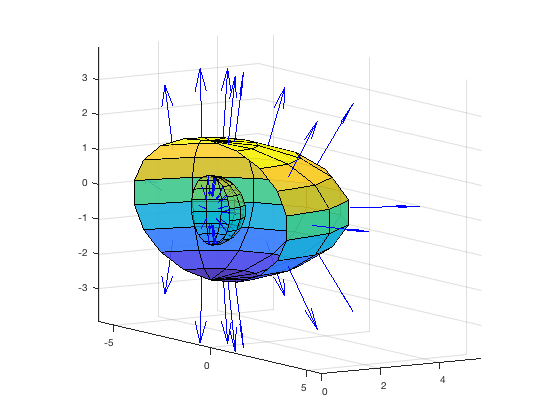
\includegraphics[width=2in]{img/C32p4-18.png}
    \vspace{1.5in}

\eject
% \noindent\textbf{Example (divergence theorem).}  Let $\displaystyle\mb F = \frac{\mb r}{\Vert\mb r\Vert^3}.$  For surface $\displaystyle S_i$, the flux out of $\displaystyle S_i$ is $\displaystyle Q_i$.  Which of the $\displaystyle Q_i$ are equal to one another?  What are the values of $Q_i$?

% \begin{enumerate}
%     \item $S_1$: sphere of radius $1$ centered at $(3,3,0)$.
%     \item $S_2$: $x^2+(y-1)^2+z^2=3$.
%     \item $S_3$: box with sides $x=\pm 2$, $y=\pm1$, $z=\pm1$.
%     \item $S_4$: box with sides $x=1,3$, $y=\pm1$, $z=\pm 1$.
%     \item $S_5$: $x^2+y^2+z^2 = 4$.
%     \item $S_6$: ellipsoid $x^2/4 + y^2+3z^2 = 1$.
% \end{enumerate}

\vspace{0.2cm}
\hrule
\vspace{0.2cm}

\noindent\textbf{Generalizing Green's theorem}. \S 20.1-20.2
\begin{tcolorbox}
\begin{itemize}
\itemsep0em
    \item \textbf{Green's theorem}: suppose $C$ is a piecewise smooth simple closed curve with $C = \partial R$.  Suppose $\mb F = P\mb i + Q\mb j$ is a smooth vector field on an open region containing $R$ and $C$.  Then $\oint_{\partial R} \mb F\cdot d\mb r = \int_R (Q_x - P_y)\ dx\ dy.$
    \item Use the notation $\text{circ}_{\mb k}\ \mb F$ to indicate the circulation density (scalar curl) of the vector field in the $xy$-plane.  $\text{circ}_{\mb k}\ \mb F = Q_x - P_y$.  $\mb k$ is indicating the axis of the circulation density.
    \item \textbf{Stokes' theorem} generalizes Green's theorem to apply to the bounding curves of regions in other planes (the $xz$-plane, the $yz$-plane, an arbitrary plane) and also to the boundary curves of non-planar piecewise smooth surfaces.
\end{itemize}
\end{tcolorbox}

\noindent\textbf{Example ($yz$-plane)}.  Suppose $R$ is a region in the $yz$-plane whose boundary is a piecewise smooth simple closed curve.  Suppose $\mb F = F_2\mb j + F_3\mb k$ is a smooth vector field on an open region containing $R$ and the boundary curve(s) of $R$, $\partial R$.  $\displaystyle\oint_{\partial R} \mb F\cdot d\mb r = \int_R \text{circ}_{\mb i}\ \mb F\ dy\ dz$ where $\text{circ}_{\mb i}\ \mb F$ is the circulation density of the vector field at a point in the $yz$-plane (with the region in the plane oriented with circulation about $\mb i$, rather than $-\mb i$.)

Thinking by analogy to the $xy$-plane, where $\text{circ}_{\mb k}\ \mb F = Q_x - P_y$, what is $\text{circ}_{\mb i}\ \mb F$?

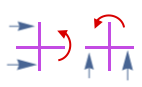
\includegraphics[width=1.5in]{img/C33p1-18.png}

%\emph{pollQ}

\vspace{1in}

\noindent\textbf{Circulation density and curl} \S 20.1
\begin{tcolorbox}
\begin{itemize}
\itemsep0em
    \item  The \textbf{circulation density} of a smooth vector field $\mb F$ at $(x,y,z)$ about the direction $\mb n$ is denoted $\text{circ}_{\mb n}\ \mb F$. 
    \item Let $\mb F = F_1\mb i + F_2\mb j + F_3\mb k$. 
    \begin{itemize}
    \itemsep0em
        \item $\text{circ}_{\mb i}\ \mb F = \partial_z F_3 - \partial_y F_2$. 
        \item $\text{circ}_{\mb j}\ \mb F = \partial_x F_1 - \partial_z F_3$. 
        \item $\text{circ}_{\mb k}\ \mb F = \partial_y F_2 - \partial_x F_1$. 
    \end{itemize}
    \item Define the curl vector, $\text{curl }\mb F = \left\langle \text{circ}_{\mb i}\ \mb F, \text{circ}_{\mb j}\ \mb F, \text{circ}_{\mb k}\ \mb F\right\rangle$.  
    \item The circulation density about the direction $\mb a = a_1\mb i + a_2\mb j + a_3\mb k$ is given by: $\text{circ}_{\mb a} \mb F = \displaystyle\frac{\mb a}{\Vert \mb a \Vert} \cdot \text{curl }\mb F$.
\end{itemize}
\end{tcolorbox}

\eject
\noindent\textbf{Circulation density and curl: implication of the dot product} \S 20.1
\begin{tcolorbox}
\begin{itemize}
\itemsep0em
    \item $\text{curl }\mb F = \nabla \times \mb F$.  This is not really a cross product (because $\nabla$ is a derivative operator, not a vector.  $\mb F\times\nabla$ is not meaningful, for example), but this shorthand allows you to compute the terms of the curl.
    \item $\displaystyle\text{circ}_{\mb n}\ \mb F = \left(\mb\nabla\times\mb F\right)\cdot \hat {\underline n} = \Vert\mb\nabla\times\mb F\Vert\cos\theta$ where $\theta$ is the angle between $\mb n$ and $\mb\nabla\times\mb F$.  When $\theta = 0$, the circulation density is maximum.  When $\theta = \pi/2$, the circulation density is zero.  When $\theta = -\pi$, the circulation density is at its minimum (and is negative).
    \item The direction of curl $\mb F(x,y,z)$ is the direction $\mb n$ for which circ$_{\mb n}$ $\mb F(x,y,z)$ is the greatest.
    \item The magnitude of curl $\mb F(x,y,z)$ is the circulation density of $\mb F$ around that direction.
    \item 
If the circulation density is zero around every direction then we define the curl to be $\mb 0$.
\end{itemize}
See \url{https://mathinsight.org/curl_subtleties} for some curl animations.
\end{tcolorbox}
\noindent\textbf{Example (computing curl)}.  Find $\mb\nabla\times\mb F$ for $\mb F = (-x+y)\mb i + (y+z)\mb j + (-z+x)\mb k$.


\begin{lstlisting}
syms x y z
curl([-x+y,y+z,-z+x],[x,y,z])
% Matlab's curl command takes two vectors as input
% the first vector is the vector field.
% The second vector is indicating the order of the coordinates.
\end{lstlisting}

\vspace{1in}

\noindent\textbf{Example (computing curl)}.  Find $\mb\nabla\times\mb F$ for $\mb F =  x\mb j + x\mb k$.

\vspace{1.5in}


\noindent\textbf{Example (curl and circulation density).}  Let $\mb F = x\mb j + x\mb k$.  The vector field is shown in blue in the figures on the left.  The red vectors are the projection of the vector field onto each surface.  The surface on the left is parallel to the $xy$-plane.  The surface on the right is the surface for which the circulation density is maximum.

\hspace{-1in}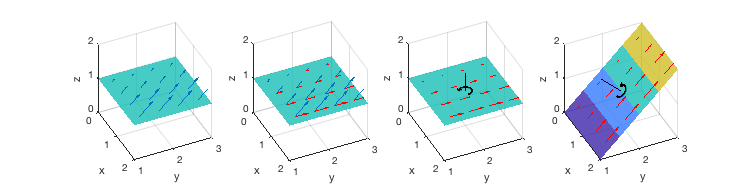
\includegraphics[width=1.2\linewidth]{img/C33p2-18.png}


\begin{enumerate}
\itemsep4em
    \item Find a vector indicating the axis about which circulation density will be maximum.  Why is the axis the same at every point $(x,y,z)$?

    \item Find an equation for a plane that has this axis as its normal vector and passes through the point $(1,2,1)$  (the plane in the plot on the right).
    \item Compare the circulation density at $(1,2,1)$ in the plane $z = 1$ to the maximum circulation density at $(1,2,1)$.
\end{enumerate}
\vspace{1in}

% \noindent\textbf{Div, grad, curl}.  Let $\mb F$ be a vector field and $f$ be a scalar function, both defined for all $(x,y,z)$.  Let $\mb r = x\mb i + y\mb j + z\mb k$.  Which of the following are not defined?
% \begin{enumerate}
%     \item curl $f$
%     \item grad $\mb F$
%     \item curl $\mb F +$ grad $f$
%     \item curl$(\mb F + $grad $f)$
%     \item $f +$ div $\mb F$
% \end{enumerate}
% \emph{pollQ}


\vspace{0.2cm}
\hrule
\vspace{0.2cm}






% \noindent\textbf{Skill Check Practice}
% \begin{questions}
% \item Compute the curl of the vector field $\mb F = \langle 3x, -5z, y\rangle$.
% \item Find the circulation density of $\mb F$ about the direction $\mb n = 2\mb i + \mb j$.

% \end{questions}

% \noindent\textbf{Skill Check Practice Solution}
% \begin{questions}
% \item 
% \begin{align*}\text{curl }\mb F &= \left\vert\begin{array}{c c c}\mb i & \mb j & \mb k \\ \partial_x & \partial_y & \partial_z \\ 3x & -5z & y\end{array}\right\vert\\
% &= \mb i(\partial_y(y) - \partial_z(-5z)) -\mb j(\partial_x(y)-\partial_z(3x)) +\mb k(\partial_x(-5z)-\partial_y(3x)) \\
% &=6\mb i\end{align*}
% \item $\hat{\underline n} = \langle 2/\sqrt{5}, 1/\sqrt{5}\rangle$.  $\text{circ}_{\mb n} \mb F = \langle 2/\sqrt{5}, 1/\sqrt{5}\rangle\cdot 6\mb i = 12/\sqrt{5}$
% \end{questions}
\end{document}